\documentclass[12pt]{article}
\usepackage[LGR, T1]{fontenc}
\usepackage[utf8]{inputenc}
\usepackage[greek,english]{babel}
\usepackage{alphabeta}
\usepackage{multicol}
\usepackage[margin=0.8in]{geometry}
\usepackage{microtype}
\usepackage{csvsimple}
\usepackage{multirow}
\usepackage{graphicx}
\usepackage{tikz}
\usepackage{hyperref}
\usepackage{algorithm} 
\usepackage{algorithmic}
\usepackage{csquotes}
\usepackage{amsmath}
\usepackage{amssymb}
\usepackage{alphabeta}
\usepackage{pgfgantt}
\usepackage{xcolor}  
\usepackage{framed}
\usepackage{listings}
\usepackage{tabularx}
\usepackage{adjustbox}
\usepackage{caption}
\usepackage{minted}
\usepackage{cite}
\usepackage{textcomp}
\usepackage{subfigure}
\usepackage{subcaption}



\title{Εργαστηριακή Άσκηση 1 \\ Πυραμίδες}
\author{Μαριάνθη Θώδη}
\date{Νοέμβριος 2025}

\begin{document}
\begin{figure}
\begin{flushleft}
  
\includegraphics[width=6cm]{logo.png}
  \hfill
\end{flushleft}
\end{figure}

\maketitle
\newpage
\tableofcontents

\section{Abstract}

\subsection{Θεωρία — Βασικές σχέσεις}
Σε αυτό το section παραθέτουμε τις βασικές μαθηματικές σχέσεις που χρησιμοποιούνται στην κατασκευή και ανάλυση Gaussian και Laplacian πυραμίδων. Οι εξισώσεις παρατίθενται σύμφωνα με τα μαθηματικά βήματα (5)–(9) από το φυλλάδιο.

\subsubsection{Γκαουσιανό Φίλτρο (1D Kernel)}

Ορίζουμε τον πυρήνα $h$ ως:
\begin{equation}
h = \frac{1}{16} [1,4,6,4,1]
\label{eq:gaussian_kernel}
\end{equation}

\textbf{Ιδιότητες:}
\begin{itemize}
    \item \textbf{Συμμετρικό:} $h[n] = h[4-n]$, δηλαδή η κατανομή είναι συμμετρική γύρω από το κέντρο. \label{eq:symmetric}
    \item \textbf{Normalized filter:} $\sum h[n] = 1$, ώστε η ένταση του σήματος να παραμένει σταθερή μετά το φίλτρο. \label{eq:normalized}
    \item \textbf{Προσέγγιση Gaussian:} Πρόκειται για binomial approximation της Gaussian συνάρτησης. Τα στοιχεία του προκύπτουν από τον διωνυμικό συντελεστή:
    \begin{equation}
    (1+1)^4 = [1,4,6,4,1]
    \label{eq:binomial}
    \end{equation}
\end{itemize}

\textbf{Σκοπός:} Το φίλτρο χρησιμοποιείται για smoothing πριν από το downsampling ώστε να μειώνεται το aliasing, δηλαδή η παραμόρφωση που εμφανίζεται όταν μειώνεται η ανάλυση.

\subsubsection{Μείωση (Reduce / Downsampling)}

Η διαδικασία μείωσης ενός σήματος $x_j[n]$ σε ένα επόμενο επίπεδο $x_{j+1}[n]$ δίνεται από:
\begin{equation}
x_{j+1}[n] = (x_j * h)[2n]
\label{eq:reduce1}
\end{equation}
ή συμβολικά:
\begin{equation}
x_{j+1} = \downarrow 2 (x_j * h)
\label{eq:reduce2}
\end{equation}

\textbf{Σημειώσεις:}
\begin{itemize}
    \item $*$ = convolution (συσχέτιση σήματος με φίλτρο)
    \item $\downarrow 2$ = κρατάμε κάθε δεύτερο δείγμα, μειώνοντας το μέγεθος κατά 2.
\end{itemize}

\textbf{Σκοπός:} Μείωση της ανάλυσης και του μεγέθους του σήματος, ενώ ταυτόχρονα διατηρούνται οι βασικές πληροφορίες μέσω smoothing.

\subsubsection{Ανάπτυξη (Expand / Upsampling)}

Η αντίστροφη διαδικασία αυξάνει την ανάλυση του σήματος $x_{j+1}[n]$ ώστε να ταιριάξει με το προηγούμενο επίπεδο $x_j[n]$:
\begin{equation}
\hat{x}_j[n] = ((\uparrow 2 \; x_{j+1}) * h')[n]
\label{eq:expand}
\end{equation}

\textbf{Σημειώσεις:}
\begin{itemize}
    \item $\uparrow 2$ = upsample (ενθέτουμε μηδενικά ανάμεσα στα δείγματα)
    \item $h' = 2h$, ώστε να διατηρείται η συνολική ενέργεια του σήματος.
\end{itemize}

\textbf{Σκοπός:} Επαναφορά του σήματος στο αρχικό μέγεθος για να υπολογίσουμε τη διαφορά Laplacian, δηλαδή τα λεπτομερή στοιχεία που χάθηκαν κατά τη μείωση.

\subsubsection{Laplacian Επίπεδο}

Κάθε επίπεδο Laplacian ορίζεται ως η διαφορά μεταξύ του τρέχοντος Gaussian επιπέδου και της επέκτασης του επόμενου επιπέδου:
\begin{equation}
L_j = x_j - \text{expand}(x_{j+1})
\label{eq:laplacian}
\end{equation}

\textbf{Σημείωση:} Περιέχει λεπτομέρειες υψηλής συχνότητας που χάνονται στο downsampling. Είναι ουσιαστικά ένα band-pass σήμα.

\textbf{Σκοπός:} Η αποθήκευση των διαφορών αυτών επιτρέπει ακριβή ανακατασκευή του σήματος ή της εικόνας αργότερα.

\subsubsection{Ανακατασκευή (Reconstruction)}

Το αρχικό σήμα $x_0$ μπορεί να ανακατασκευαστεί από την Laplacian πυραμίδα $L_j$ και το τελευταίο Gaussian επίπεδο $x_L$:
\begin{equation}
x_0 = \sum_{j=0}^{L-1} \text{expand}^{(j)}(L_j) + \text{expand}^{(L)}(x_L)
\label{eq:reconstruction}
\end{equation}

\textbf{Σημειώσεις:}
\begin{itemize}
    \item Επεκτείνουμε κάθε Laplacian επίπεδο στην αρχική ανάλυση.
    \item Προσθέτουμε όλα τα επίπεδα μαζί με το coarsest Gaussian $x_L$.
    \item Η διαδικασία διατηρεί την πληροφορία του αρχικού σήματος (εκτός από αριθμητικά σφάλματα).
\end{itemize}

\subsubsection{Σχέσεις μεταξύ Εξισώσεων}

\begin{itemize}
    \item \textbf{Reduce → Expand:} 
    \begin{equation}
    \text{expand}(\text{reduce}(x)) \approx x
    \label{eq:reduce_expand}
    \end{equation}
    αν το φίλτρο είναι σωστά σχεδιασμένο.
    
    \item \textbf{Gaussian → Laplacian:} 
    \begin{equation}
    L_j = x_j - \text{expand}(x_{j+1})
    \label{eq:gaussian_laplacian}
    \end{equation}
    
    \item \textbf{Laplacian → Gaussian:} 
    \begin{equation}
    x_0 = \sum_j \text{expand}^{(j)}(L_j) + \text{expand}^{(L)}(x_L)
    \label{eq:laplacian_gaussian}
    \end{equation}
\end{itemize}

\textbf{Συμπέρασμα:} Ο κύκλος Gaussian → Laplacian → Gaussian αποτελεί τη βάση για τις πυραμιδικές αναπαραστάσεις, που χρησιμοποιούνται σε blending εικόνων και άλλες εφαρμογές επεξεργασίας εικόνας.

\subsection{Επιβεβαίωση Gaussian Πυρήνα}

\paragraph{1. Θεωρητική εξήγηση}
\paragraph{Δυωνυμικός πυρήνας $h$}

Ο πυρήνας
\[
h = \frac{1}{16}[1, 4, 6, 4, 1]
\]
είναι ένας 5-σημείων δυωνυμικός πυρήνας, προερχόμενος από το τρίγωνο του Pascal (διωνυμικοί συντελεστές της τάξης 4).  

Η κανονικοποίηση διατηρεί τη συνολική ένταση του σήματος:
\[
\sum h[n] = 1.
\]

Οι δυωνυμικοί πυρήνες αποτελούν διακριτές προσεγγίσεις του Γκαουσιανού φίλτρου, και σύμφωνα με το Κεντρικό Οριακό Θεώρημα, όταν το μήκος του πυρήνα αυξάνεται ($N \to \infty$), ο δυωνυμικός πυρήνας συγκλίνει σε συνεχή Gaussian.  

Για πρακτικούς σκοπούς, το $h$ μπορεί να θεωρηθεί διακριτό Γκαουσιανό φίλτρο.  

Η συνέλιξη με τον δυωνυμικό πυρήνα εξομαλύνει ένα σήμα όπως ένα Gaussian φίλτρο, κάνοντας μέσο όρο τις γειτονικές τιμές και μειώνοντας τον θόρυβο υψηλής συχνότητας.

\paragraph{2. Σχέση με smoothing / χαμηλοπερατότητα}

Ο δυωνυμικός πυρήνας λειτουργεί ως χαμηλοπερατό φίλτρο:

\begin{itemize}
    \item Διατηρεί τις χαμηλές συχνότητες του σήματος.
    \item Μειώνει τις υψηλές συχνότητες, μειώνοντας aliasing πριν το downsampling.
    \item Επιτρέπει ακριβή ανακατασκευή μέσω της Laplacian πυραμίδας.
\end{itemize}

Αυτό συνδέεται άμεσα με τις πράξεις Reduce/Downsampling και Expand/Upsampling των Gaussian \& Laplacian πυραμίδων.

\paragraph{3. Οπτική σύγκριση με Gaussian}

Μπορούμε να συγκρίνουμε το $h$ με ένα Gaussian φίλτρο στο MATLAB χρησιμοποιώντας την εντολή:

\begin{verbatim}
G_fspecial = fspecial('gaussian',[1 5],1);
\end{verbatim}

Το \texttt{fspecial('gaussian')} δημιουργεί έναν 5-σημείων Gaussian πυρήνα με τυπική απόκλιση 1 και κανονικοποιημένο άθροισμα 1.  

Η σύγκριση δείχνει ότι:
\begin{itemize}
    \item Το σχήμα του δυωνυμικού πυρήνα  προσεγγίζει πολύ καλά την καμπύλη της γκαουσιανής στο χρόνο, καθιστώντας τον διακριτή προσέγγιση του Gaussian.
    \item Η frequency response μέσω fft  δείχνει ότι το φίλτρο συμπεριφέρεται χαμηλοπερατά, όπως ένα Gaussian φίλτρο.
\end{itemize}


\begin{figure}[h!]
\begin{center}
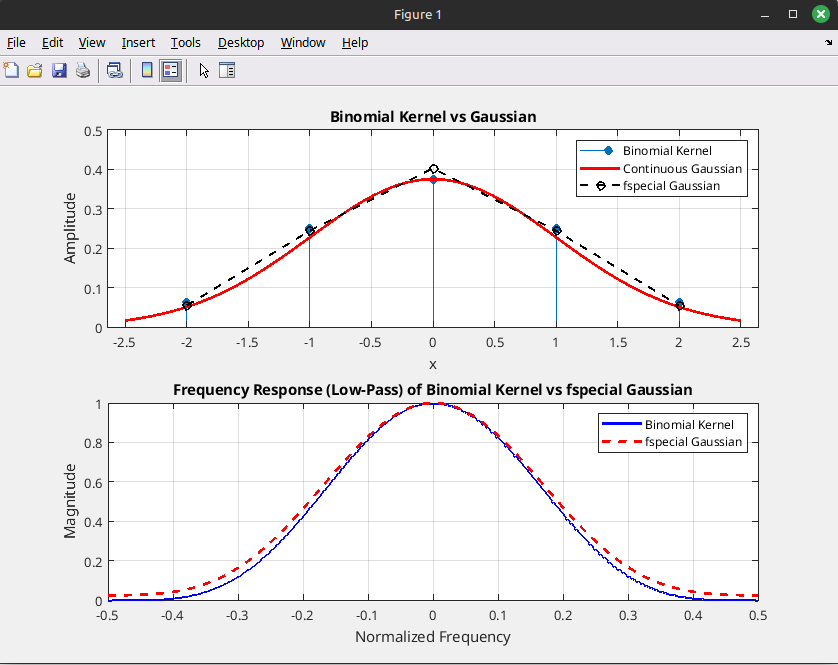
\includegraphics[width=10cm]{gaussian.png}
\caption{Plots that shows that binomial kernel approximates the gaussian filter}
\label{fig:drlagent}
\end{center}
\end{figure}

\subsubsection{Γκαουσιανή Πυραμίδα}
Η Gaussian πυραμίδα δημιουργείται για 1D σήματα $x_0, x_1, \dots, x_L$ εφαρμόζοντας τις βασικές σχέσεις \eqref{eq:gaussian_kernel}–\eqref{eq:laplacian} της θεωρίας.

\paragraph{Συνέλιξη με Gaussian πυρήνα} \mbox{} 
Ο πυρήνας 
\[
h = \frac{1}{16}[1,4,6,4,1]^T
\]
εξομαλύνει το σήμα πριν από τη μείωση (reduce), μειώνοντας τις υψηλές συχνότητες και περιορίζοντας το aliasing (βλ. \eqref{eq:gaussian_kernel}, \eqref{eq:binomial}).

\paragraph{Downsampling (Reduce)} \mbox{} 

Διατηρούμε κάθε δεύτερο δείγμα του φιλτραρισμένου σήματος για να μειωθεί η διακριτική ανάλυση κατά 2 (βλ. \eqref{eq:reduce1}, \eqref{eq:reduce2}).

\paragraph{Toeplitz Matrix}\mbox{} 

Ο Toeplitz πίνακας χρησιμοποιείται για να υλοποιηθεί η συνέλιξη μέσω γραμμικού πολλαπλασιασμού.  
Κάθε γραμμή του πίνακα είναι μια μετατόπιση του Gaussian φίλτρου.  
Ο γραμμικός συνδυασμός των στοιχείων κάθε γραμμής με τα αντίστοιχα δείγματα του σήματος δίνει το αποτέλεσμα της συνέλιξης:
\[
y = T \cdot x
\]
Αυτό αντιστοιχεί στις εξισώσεις \eqref{eq:reduce1} και \eqref{eq:reduce2}.

\paragraph{Downsampling με DN}\mbox{} 

Το DN matrix επιλέγει τα δείγματα που θα κρατηθούν μετά τη συνέλιξη:  
έχει μονάδες στις θέσεις των στοιχείων που θα διατηρηθούν και μηδενικά αλλού.  
Η εφαρμογή του στο φιλτραρισμένο σήμα μειώνει το μέγεθος κατά 2, αντιστοιχώντας στο σύμβολο ↓2 στις εξισώσεις \eqref{eq:reduce2}.

\paragraph{Kronecker Product}\mbox{} 
\
Στη 1D περίπτωση δεν χρησιμοποιείται άμεσα.  
Γενικά, μπορεί να εφαρμοστεί για διεύρυνση του DN ή για 2D συνελίξεις, όπου η εφαρμογή είναι separable κατά γραμμές και στήλες.

\paragraph{Δημιουργία Gaussian Πυραμίδας}\mbox{} 

Η συνάρτηση \texttt{gaussianPyramid(x,L)} επαναλαμβάνει:
\begin{enumerate}
    \item Συνέλιξη με Gaussian φίλτρο (Toeplitz) → smoothing (\eqref{eq:gaussian_kernel}, \eqref{eq:binomial})
    \item Downsampling με DN (\eqref{eq:reduce1}, \eqref{eq:reduce2})
    \item Αποθήκευση κάθε επιπέδου $x_j$ στο cell array $G\{j\}$
\end{enumerate}
Το αρχικό σήμα είναι το επίπεδο 0 ($x_0$). Κάθε επόμενο επίπεδο $x_{j+1}$ είναι πιο ομαλό και μικρότερο σε μέγεθος.

\paragraph{Εφαρμογή σε παράδειγμα 1D σήματος}\mbox{} 

Χρησιμοποιήθηκε το σήμα:
\[
x = \sin(2t) + 0.5 \sin(5t), \quad t \in [0,2\pi], \quad N=64
\]
Δημιουργήθηκαν 5 επίπεδα πυραμίδας ($x_0$ έως $x_4$).  
Σε κάθε επίπεδο εφαρμόζεται πρώτα το φίλτρο και μετά το downsampling, σύμφωνα με τις εξισώσεις \eqref{eq:reduce1}–\eqref{eq:reduce2} και παρατίθονται τα plots παρακάτω.


\begin{figure}[h!]
    \begin{center}
    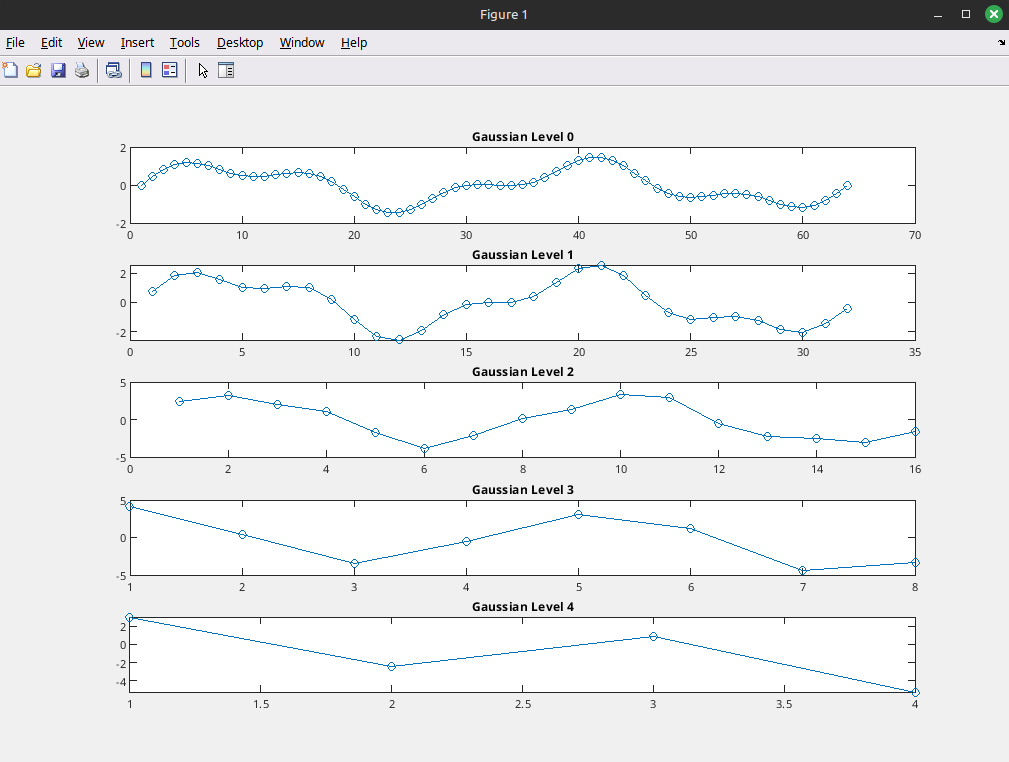
\includegraphics[width=10cm]{gaussian1D.png}
    \caption{Gaussian πυραμίδα 1D: κάθε επίπεδο δείχνει το σήμα μετά Gaussian φίλτρο και downsampling}
    \label{fig:drlagent}
    \end{center}
    \end{figure}

\paragraph{Εξήγηση των Plots}\mbox{} 

Στα plots παρουσιάζονται όλα τα επίπεδα της Gaussian πυραμίδας:
\begin{itemize}
    \item \textbf{Επίπεδο 0:} Το αρχικό σήμα με όλες τις συχνότητες.
    \item \textbf{Επίπεδα 1–4:} Το σήμα γίνεται σταδιακά πιο ομαλό λόγω του Gaussian φίλτρου. Η διακριτική ανάλυση μειώνεται επειδή διατηρούμε κάθε δεύτερο δείγμα.  
    Τα plots δείχνουν οπτικά τη διαδικασία smoothing και υποδειγματοληψίας, όπως περιγράφεται στις εξισώσεις \eqref{eq:reduce1}–\eqref{eq:reduce2}.
\end{itemize}

Η διαδικασία αυτή αποτελεί τη βάση για την κατασκευή Laplacian πυραμίδων (\eqref{eq:gaussian_laplacian}) και τελικά την ανακατασκευή του σήματος (\eqref{eq:reconstruction}).  

Η ίδια λογική μπορεί να εφαρμοστεί σε 2D εικόνες με separable convolution: πρώτα κατά γραμμές, μετά κατά στήλες.



\section{Μέρος 2 — Συρραφή εικόνων με Λαπλασιανές Πυραμίδες}



\section{Μέρος 3 — Δημιουργία Σύνθεσης πολλών εικόνων}


\section{Μέρος 4 — Semantic Segmentation με PSPNet}








\end{document}